\chapter{Effect of Added Body Mass on Maximal Power Output During Cycling}
\label{Chap:C}
\pagestyle{headings}

\section{Abstract}


\section{Introduction}
If riders use the inertia of their CoM to amplify instantaneous crank power during maximal sprints in a non-seated posture, then increasing the inertia of the CoM should increase the magnitude of power amplification. One way to increase inertia of the rider's CoM is to add mass to the torso. Thus, if a rider can generate enough power on the additional mass, then theoretically the additional mass should increase the instantaneous crank power that a rider can produce during maximal sprinting in a non-seated posture and perhaps even in a seated posture.  

\section{Materials and methods}
\subsection{Participants}
Three people (2M; 1F, age = $\pm$, height = $\pm$, mass = $\pm$) volunteered to take part in this study.

\subsection{Experimental design}
Participants began with a 5-min cycling warm-up at 100 W at their preferred cadence. Participants then performed a total of eight 5-s maximal sprints on an instrumented ergometer (Excalibur Sport, Lode BV, Groningen, The Netherlands) in a seated or non-seated posture either with or without added torso mass, which was equal to 20$\%$ of the rider's body mass. Given that rider still needs to be able to move their CoM to generate power, we estimated that 20$\%$ of body mass would be heavy enough for us to detect a signal and light enough that the rider could still raise and lower their torso during each crank cycle. Full body motion capture was recorded at 200 Hz (8x Oqus, Qualisys, AB, Sweden) and crank angle, crank radial force, and crank tangential force were recorded at 100 Hz (Axis, Swift Performance, Brisbane, Australia). The ergometer was set to ``isokinetic'' mode, which ensured that cadence was kept constant at 120 rpm, which was predicted to elicit near maximal power in each participant \cite{McCartney1983}. A scaled, full-body OpenSim model was used to solve inverse kinematics and inverse dynamics \cite{Rajagopal2016}. Crank length was constant at 175 mm. Participants wore a standardised model of cleated cycling shoe (SH-R070, Shimano, Osaka, Japan) that clipped into the pedals (SH-R540, Shimano, Osaka, Japan).

\begin{figure}[htbp]
    \centering
    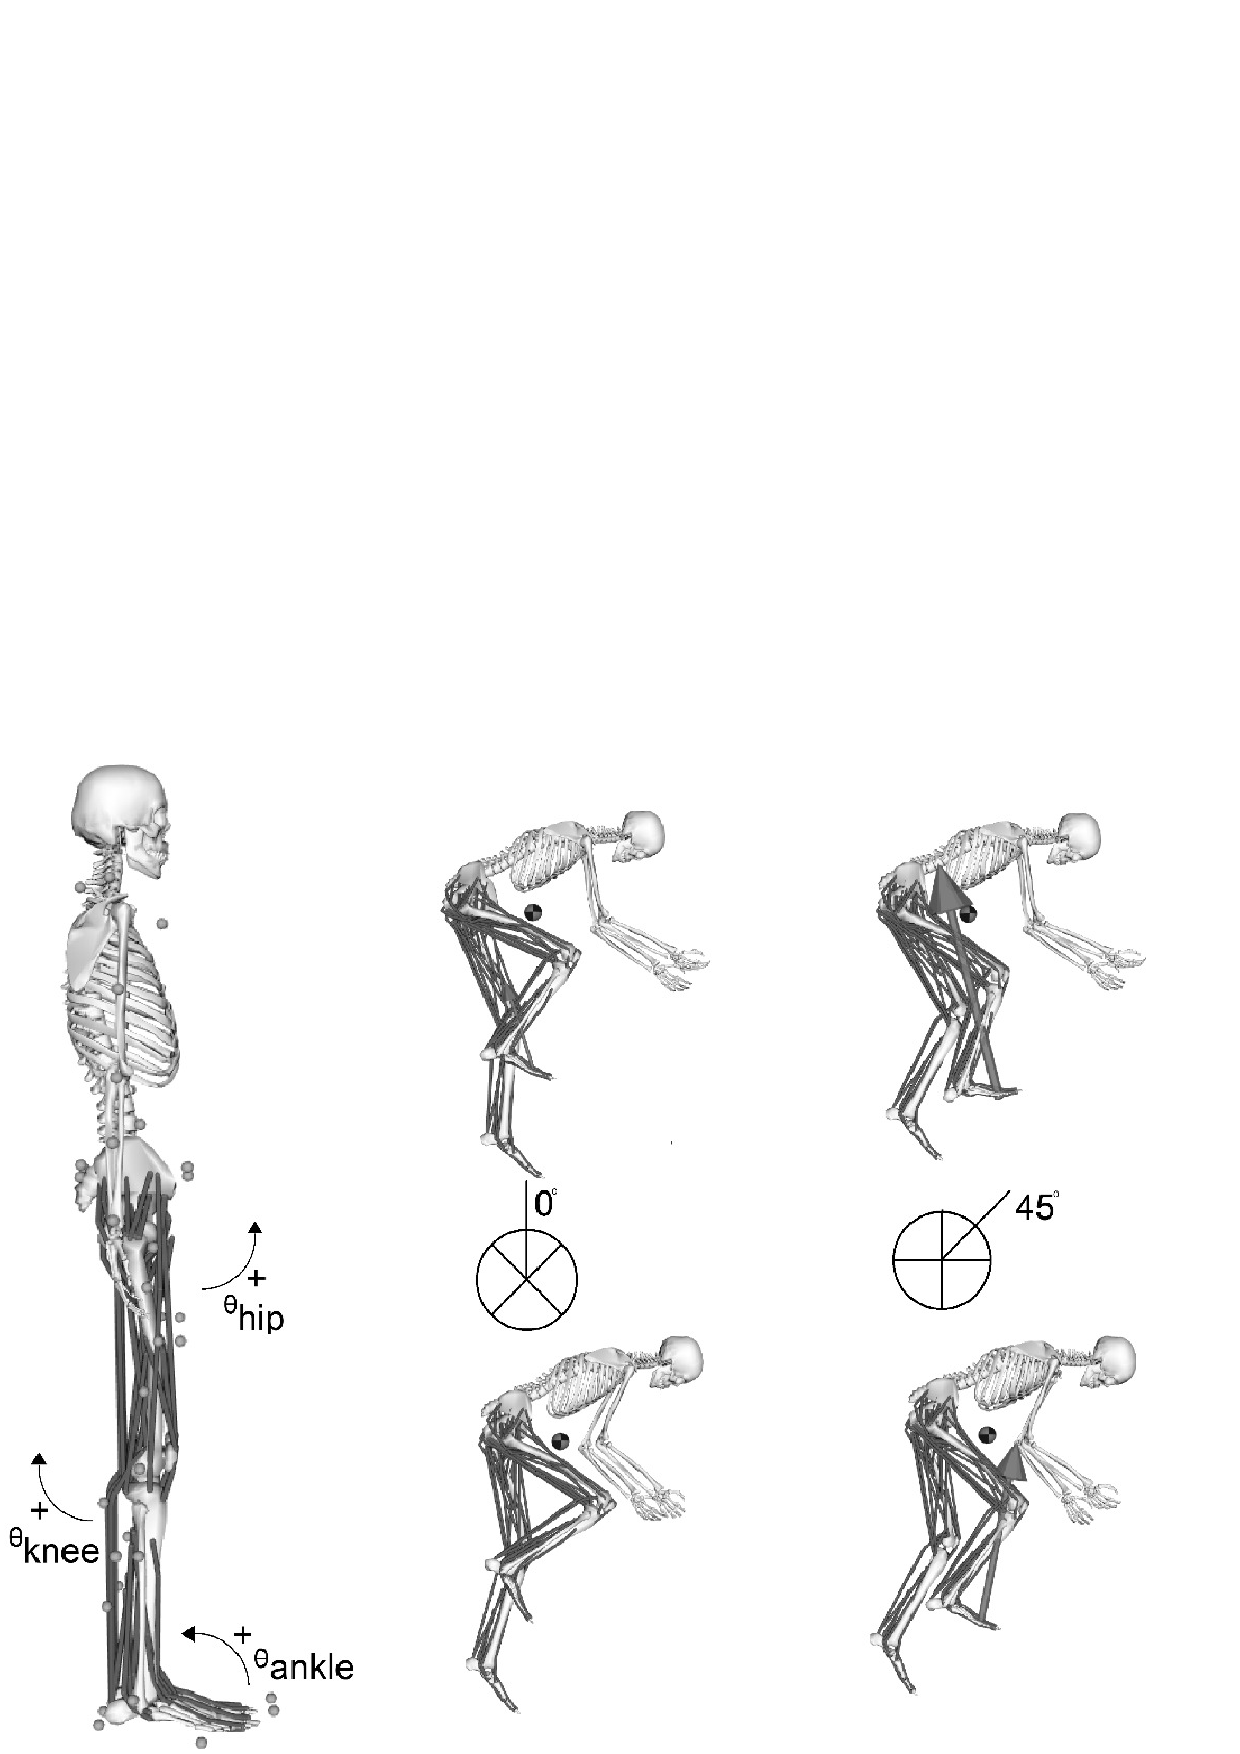
\includegraphics[width=0.6\textwidth]{Study6/Figure1.png}
    \caption[Riders were asked to perform 5-s maximal sprints at 120 rpm in a seated and non-seated posture either with or without wearing a weight vest equal to 20$\%$ of their body mass.]{\textbf{Riders were asked to perform maximal sprints at 120 rpm in a seated and non-seated posture either with or without wearing a weight vest equal to 20$\%$ of their body mass.} The vest has 10 slots on the front and back which hold 1 kg weights. A thick velcro strap was secured tightly around the vest to prevent it from wobbling vertically and horizontally during the maximal sprints.}
    \label{fig:mass1}
\end{figure}

\FloatBarrier

\section{Results}
TBC

\section{Discussion}
TBC
